\section{Results from the Tritiated Methane Calibration}



\subsection{Definition of Electronic Recoil Band and Comparison with NEST Model}

The purpose of using the tritium calibration source was to get a handle on the electronic recoil (ER) band in the fiducial volume of the LUX detector. Separating ER and nuclear recoil (NR) events is crucial for background discrimination, unfortunately it is difficult to characterize low energy ER events with external calibration sources due to the self shielding properties of liquid xenon. Here we present the results of the ER band obtained from the beta decay of tritium, uniformly distributed, in comparison to the NEST simulation prediction at an extraction field of 120 V/cm. A key parameter obtained from the ER and NR band is the leakage fraction which gives a rough measure of background rejection, for the current data set the NEST model along with AmBe and Cf neutron sources was used to define the NR band.

Leakage fraction is defined as the fraction of events in the ER band that spill into the lower half of the NR band. Tritium events are selected with standard WIMP search cuts using pulse classification, pulse pairing and the a quality cut. Two methods were used to calculate the leakage fraction. First, a cut and count in which the number of tritium events populating the lower half of the NR band are compared to the total number of tritium events in the selected S1 range. Iuring the 24 hour acquisition of the tritium data used to define the ER band there was an expectation of just one event being non tritium, thus the cut and count method is valid in this case. The second method is to assume that the ER and NR bands are gaussian and calculate their overlap. $\rm (1-erf((Mean\_ER-Mean\_NR)/(sqrt(2)*sigma\_ER)))/2 $. Both methods yield good agreement which indicated that the distribution of ER events is mostly Gaussian. Figure \ref{fig:Leak_wo_200} shows the leakage fraction per 2 Phe bins in S1. The mean leakage fraction from 0-30 Phe in the fiducial region is 0.36\% $\rm \pm$ 0.01\%, see Figure \ref{fig:Leak_wo_200}.


\begin{figure}[H]\centering
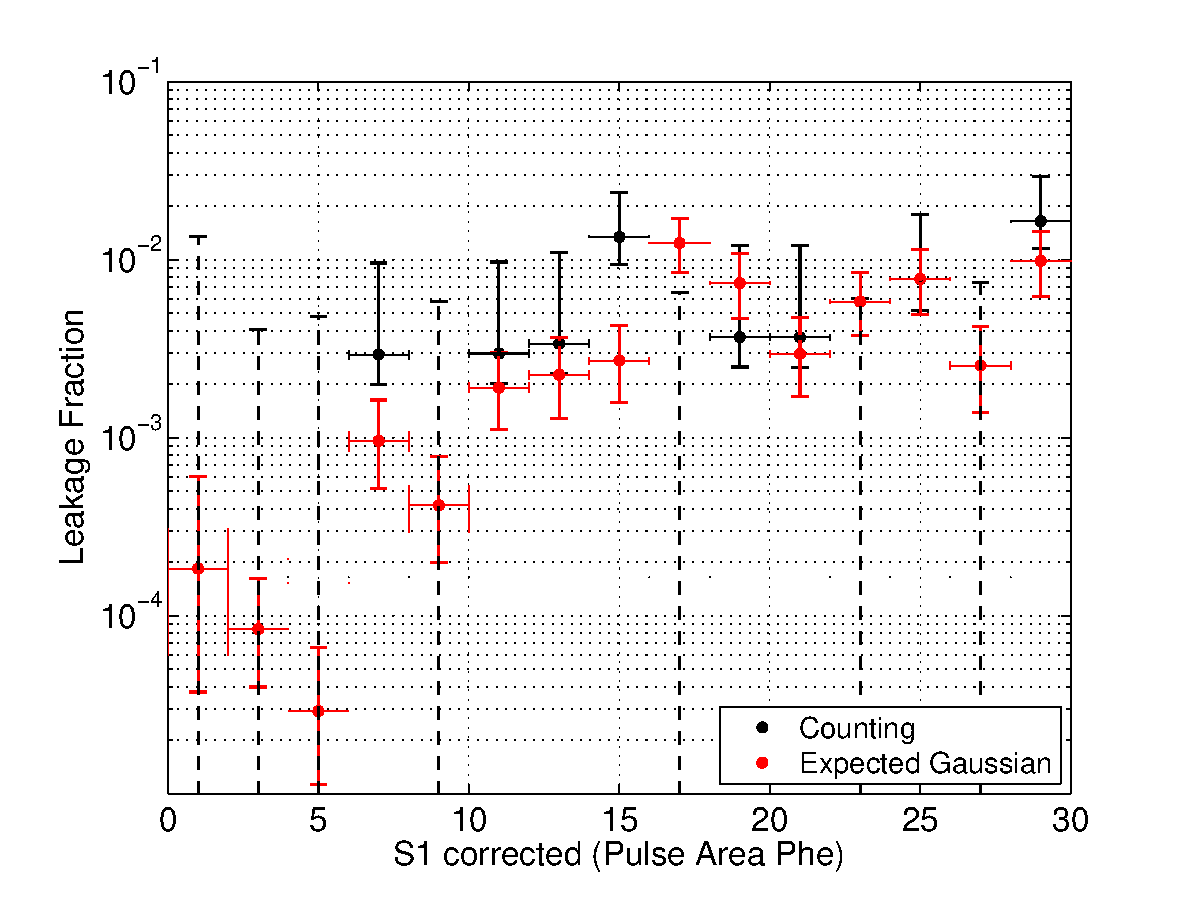
\includegraphics[width=80mm]{CH3T_Leakage_fid_30_lux10_20130813T1120_cp05328_wo200cut_note.eps}
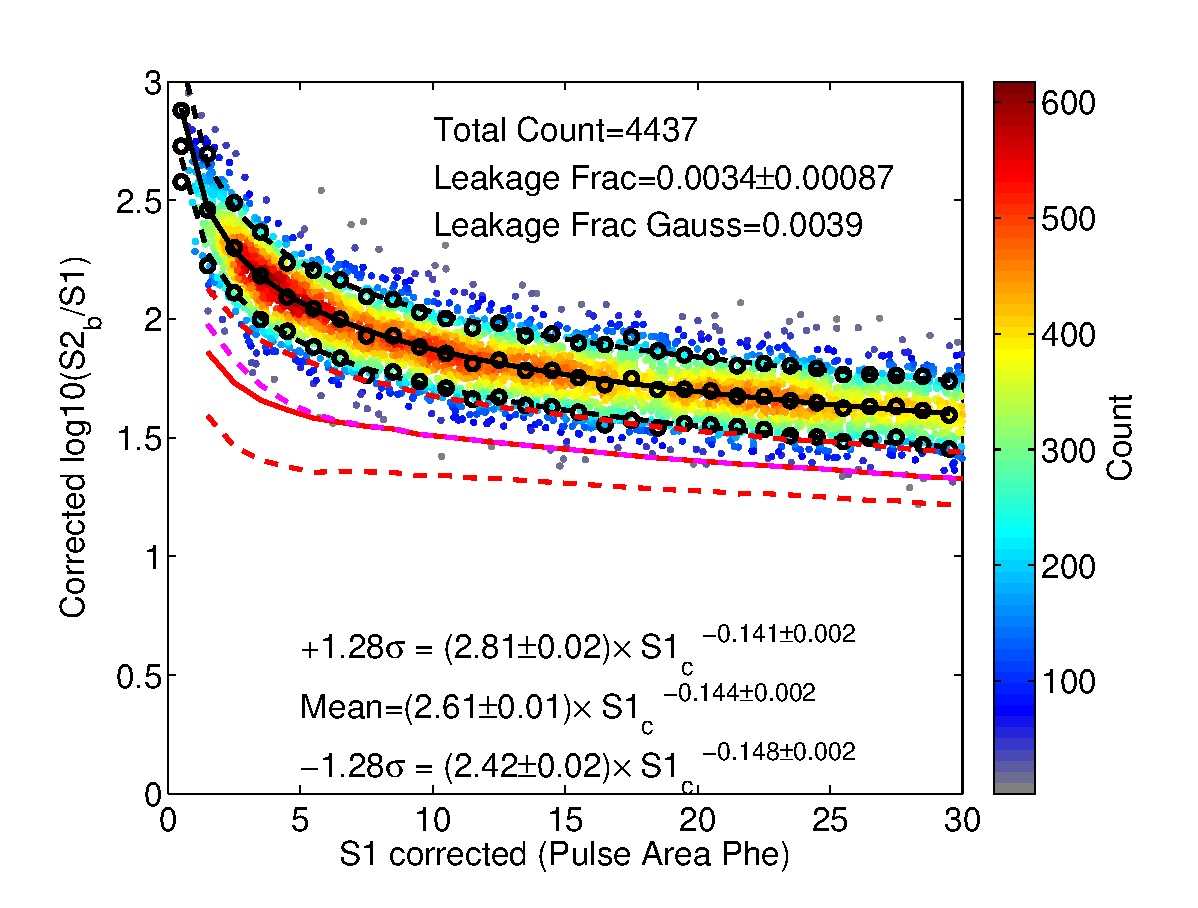
\includegraphics[width=80mm]{CH3T_fid_30_lux10_20130813T1120_cp05328_wo200cut_note.eps}
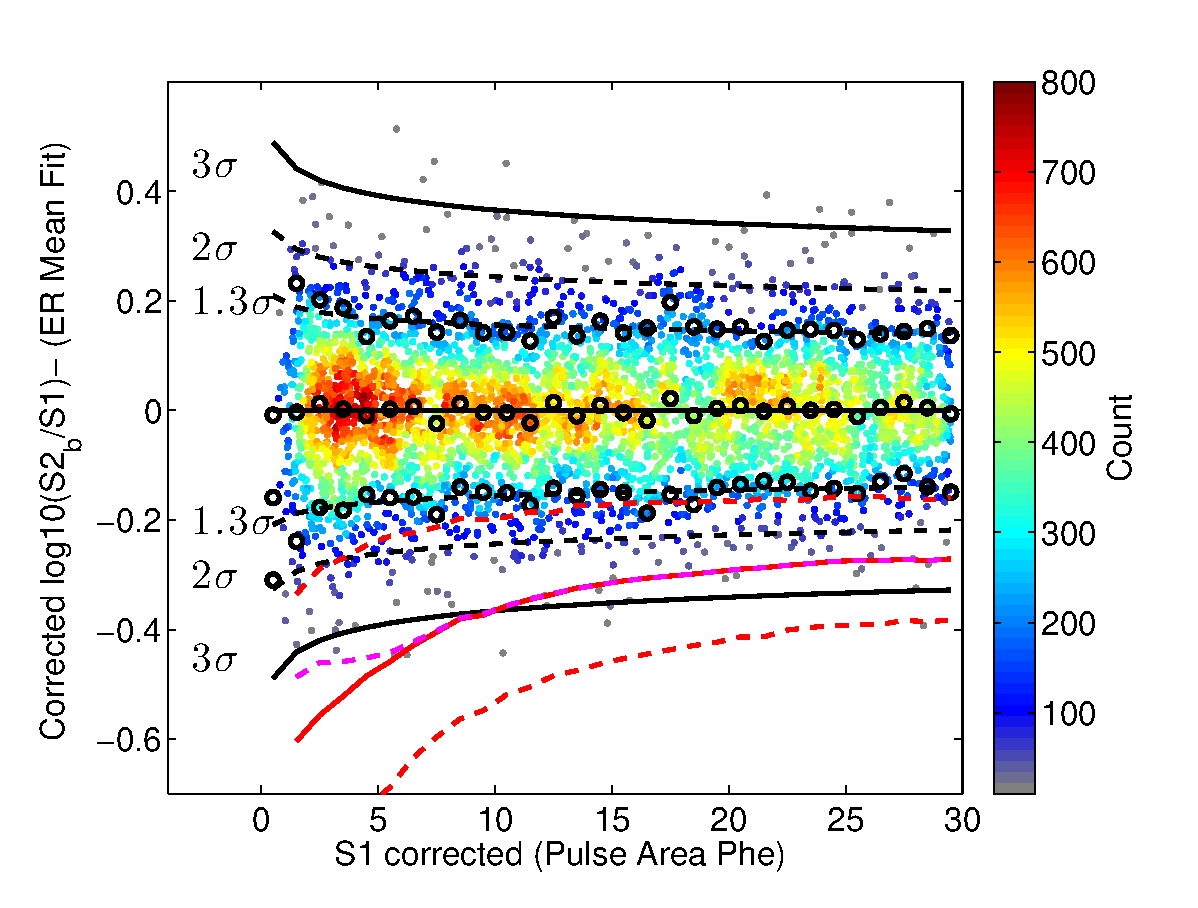
\includegraphics[width=80mm]{CH3T_fid_30_zoom_lux10_20130813T1120_cp05328_wo200cut_note.eps}
\caption{Top Left: Black, Leakage fraction calculated from cut and count. Red, leakage fraction expected from a Gaussian distribution. From 0 to 30 Phe with 2 Phe wide bins and not using the S2 $>$ 200 Phe cut. Top Right: Log(S2/S1) vs. S1 with ER band fit from the tritium data (S1: 0 to 30 Phe). Bottom. The data and fits renormalized to the ER band mean (S1: 0 to 30 Phe). The dashed magenta line is the NR mean with the S2$>$200 Phe cut (using NEST 4-b for NR).}
\label{fig:Leak_wo_200}
\end{figure}


Figure \ref{fig:NEST_v_Data} shows the comparison between simulation(NEST) and the data for the ER band. The agreement between simulation and data is good down to five phe in S1. At low energies, sub 2 keVee, the NEST model had not been vetted. The tritium data was ultimately used to define the ER band for the WIMP search run due to its high statistical significance. The newly acquired data was used to define a new NEST model that better reproduces the width and mean of the ER band at the extraction field of 120 V/cm.

\begin{figure}[H]\centering
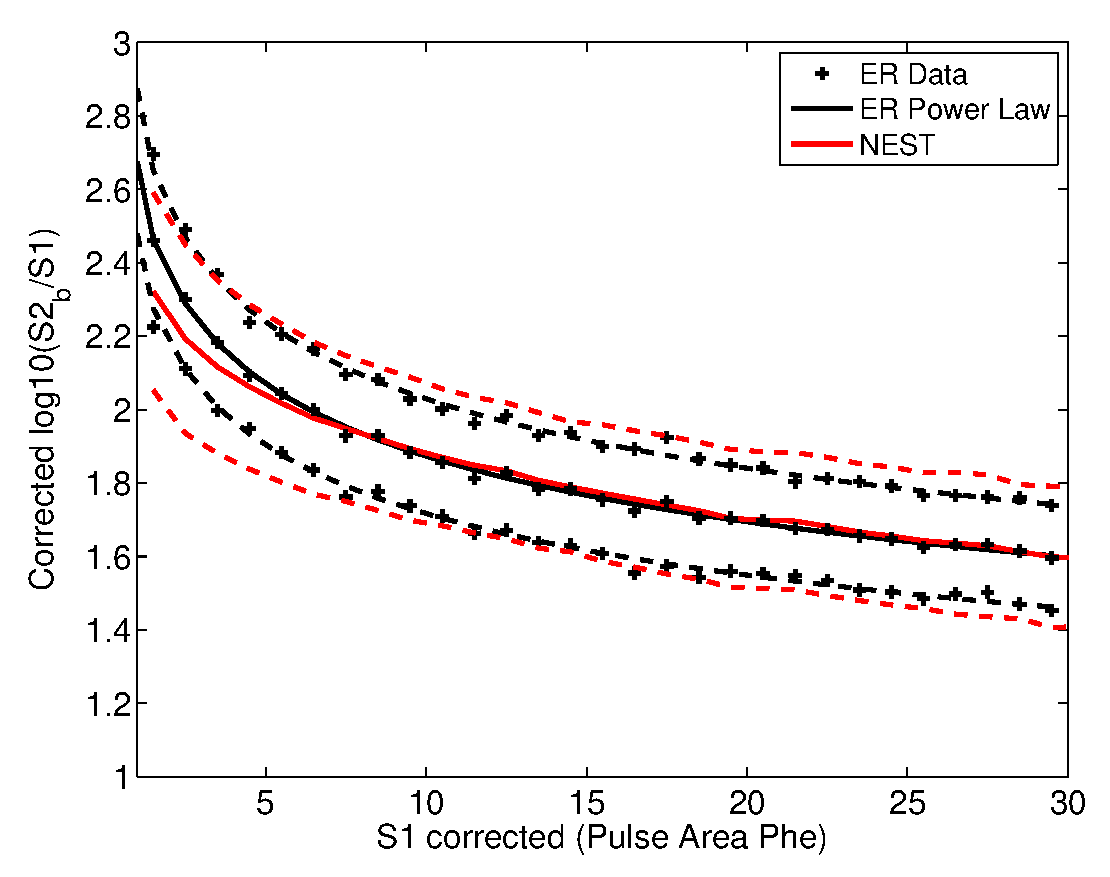
\includegraphics[width=80mm]{CH3T_DATA_NEST_fid_30_lux10_20130813T1120_cp05328.eps}
\caption{ER band from tritium data with $\rm \pm 1.3 \sigma$ (black) compared with NEST simulation prediction (Red).}
\label{fig:NEST_v_Data}
\end{figure}


\subsection{Distribution of Tritiated Methane}

 Tritium events appear uniformly distributed in the detector thirty minutes after the triturated methane injection. Figure \ref{fig:Density} shows the Z, XY and radial distribution of tritium events after an injection. When considering the tritium events a drift time cut from 5 to 324 $\mu s$ was made to cover only the region from the gate to the cathode, excluding the region between the gate and anode. An additional cut requiring that the event be between $\rm \pm 2 \sigma$ of the ER mean was made to minimize the leakage of residual alphas from the walls and cathode. The tritiated methane quickly dispersed throughout the liquid decaying in all regions on the detector, proving to be an ideal low energy calibration source.
 
\begin{figure}[H]\centering
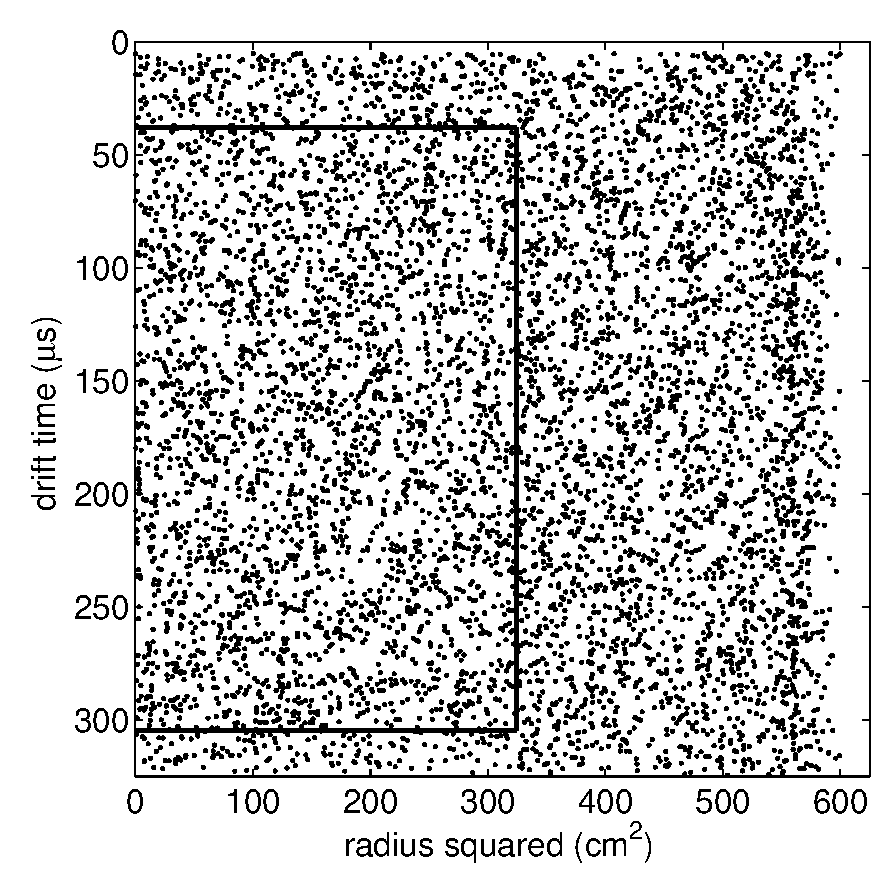
\includegraphics[width=80mm]{CH3T_RZ_scatter_lux10_20130812T1546.eps}
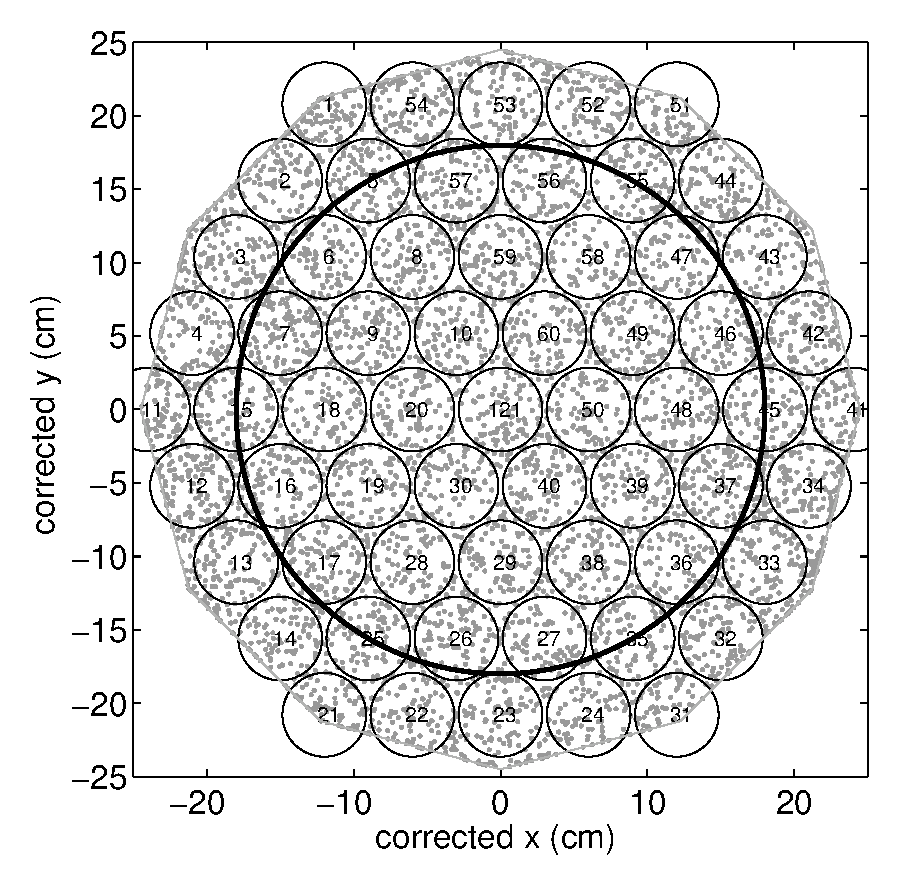
\includegraphics[width=80mm]{CH3T_XY_scatter_PMT_lux10_20130812T1546.eps}
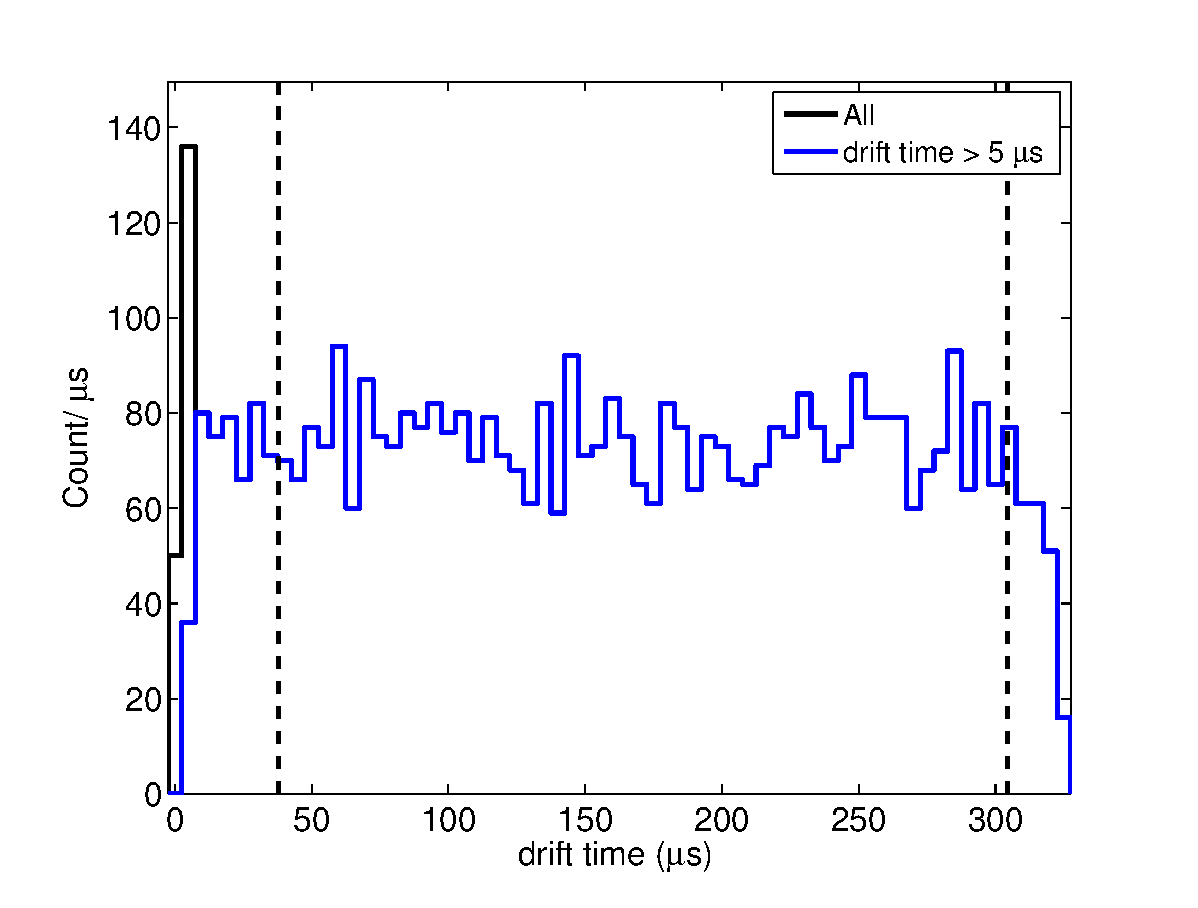
\includegraphics[width=80mm]{CH3T_Z_density_lux10_20130812T1546.eps}
\caption{Top Left: The distribution of tritium events vs. corrected radius squared. Top Right: The distribution of tritium events vs. XY-corrected in the region between the gate and the cathode, as reconstructed by the Mercury algorithm (used for LUX position reconstruction). Bottom: Distribution of tritium events vs. drift time (depth).}
\label{fig:Density}
\end{figure}

\subsection{Combined Energy Calibration}

To transform S1\_Phe and S2\_Phe to absolute energy we use a model that uses the number of quanta produced as its input, Ref[]. 
$ \rm E(s1,s2) = S1/PDE * S2/(extraction eff * single-electron-size) $. The single electron size was calculated to be 10.57 Phe, the extraction efficiency for elections was calculated to be 0.65 and the photon detection efficiency (PDE) was calculated to by 0.14.


The agreement between that data and SIM indicate that we have a good understanding of our absolute energy scale down to 2 $\rm keV_{ee}$. Between 1 and 2 $\rm keV_{ee}$ there is a region with excess events, this is likely an indication that the model used for determining energies is breaking down and needs further investigation.

\begin{figure}[H]\centering
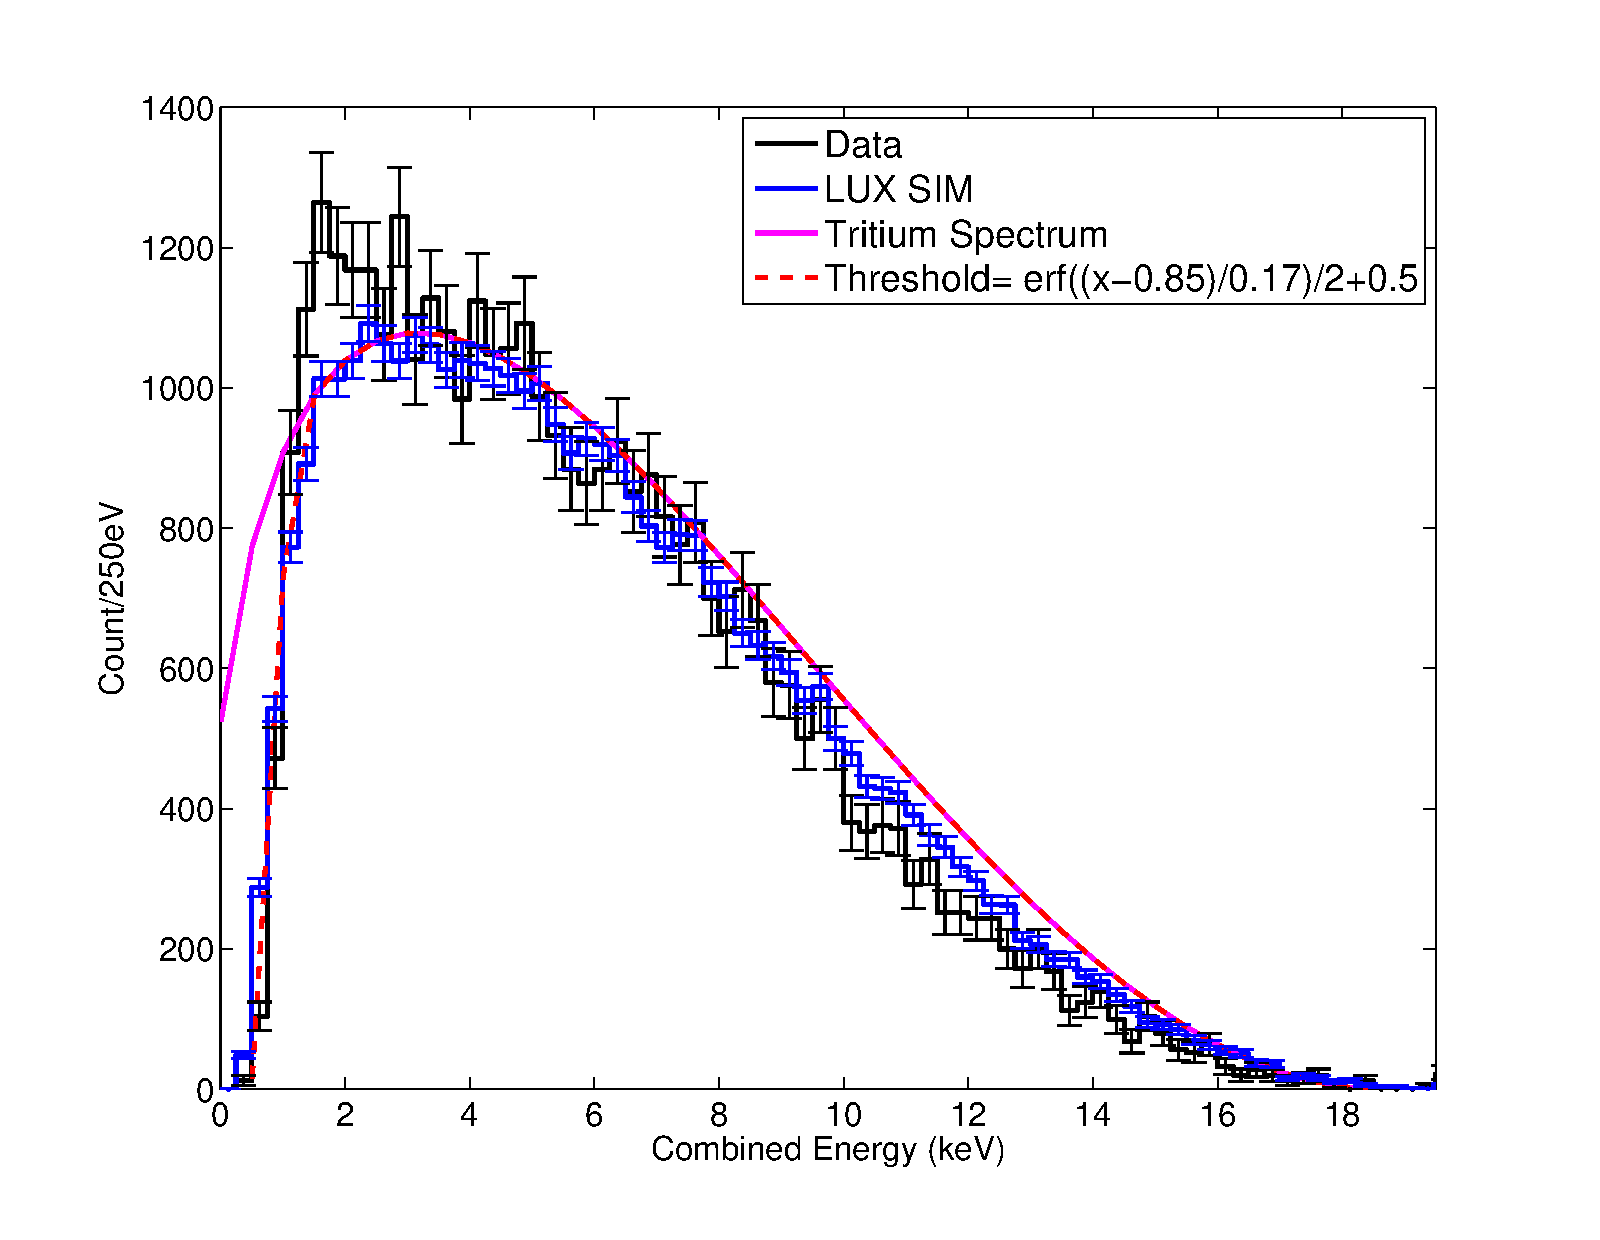
\includegraphics[width=80mm]{CH3T_E_spec_18_lux10_20130813T1120_cp05328_note.eps}
\caption{Combined energy spectrum of the Data, LUX SIM and Raw NEST model for tritium beta decay. Note, Raw NEST is with photon and electron propagation turned off which represents the tritium beta spectrum before smearing due to detector resolution.}
\label{fig:E_spec}
\end{figure}
 
 
 \subsection{Absolute Rate}
 
The absolute efficiency for detecting tritium events can be determined by comparing the number of observed events to the number expected. The initial activity injected was calculated to be $0.84 \pm 0.22 $ Bq, with the largest uncertainty coming from the ratio of $\rm CH_3T/CH_4$ from the tritiated methane source bottle. The purification time constant was measured to be 6.6 hours. From the initial rate and the purification constant we expect to count a total of $20,200 \pm 4,000 $ events in the LUX detector before applying the S1 threshold. With the S1 threshold we expect  $16,000 \pm 3,100 $ `golden' events. The actual count observed in the liquid xenon volume was 20,000 events, which is in good agreement with the expected value taking into account the uncertainty in the initial activity and the purification model. After making fiducial cut $7,700 \pm  1,500$ events were expected,  roughly $16,000 \pm  3,100 * (290/324)*(18^2/24.5^2)$. And a total of $9,500 \pm 100$ were observed, see Figure \ref{fig:Count}.

\subsection{Data vs. SIM}

The SIM contained a total of 200,000 tritium events but after WIMP search cuts there remained 156,000 due to the S1 threshold. The overall scaling between the LUX\_SIM and the Data was expected to be 156,000 events total in SIM and 20,000 in Data (for golden events), this corresponds to a factor of 1/7.8 for Data/Sim. The best fit to the S2 spectrum was found to be 1/7.9 and the best fit to the energy spectrum was found to be 1/7.5, both in good agreement with the expected rate.
 

\begin{figure}[H]\centering
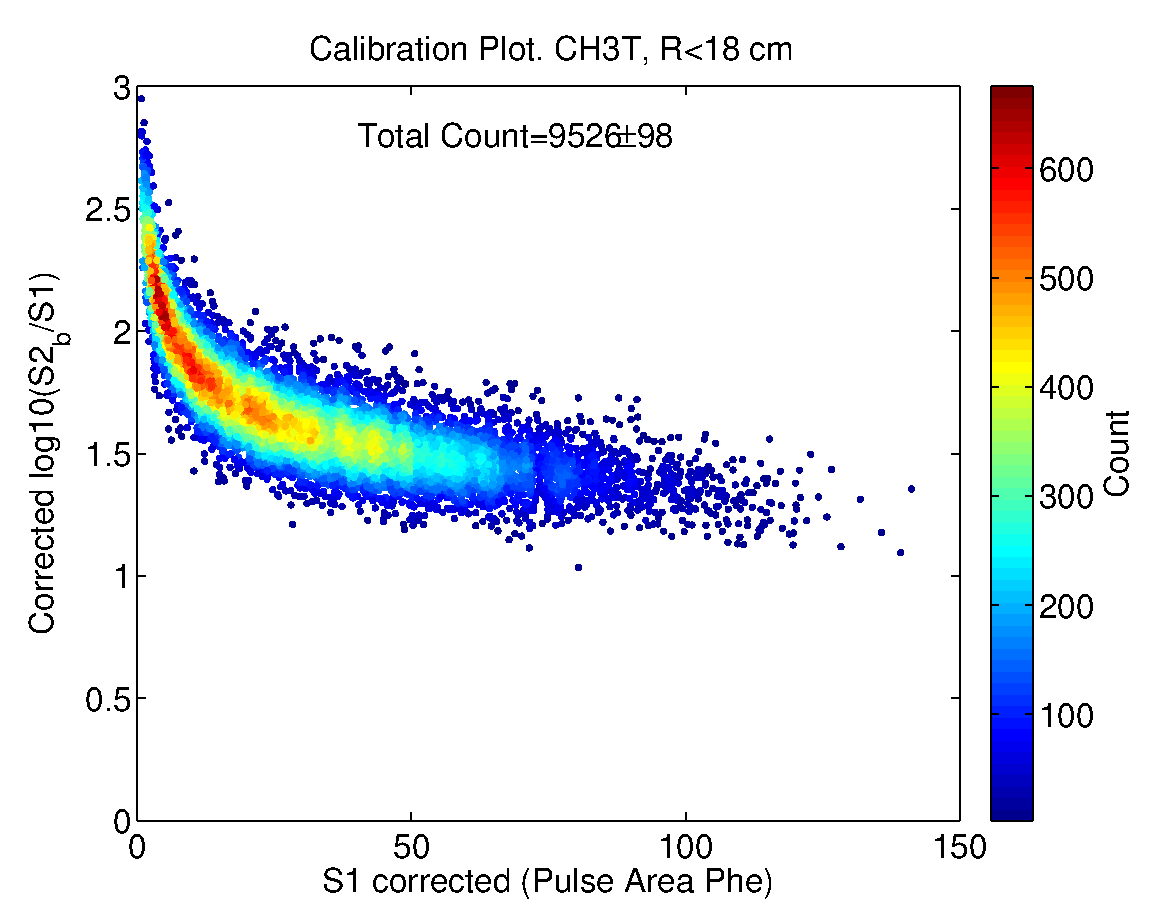
\includegraphics[width=80mm]{CH3T_all_lux10_20130813T1120_cp05328.eps}
\caption{Combined energy spectrum of the Data, LUX SIM and Raw NEST model for tritium beta decay.}
\label{fig:Count}
\end{figure}


